\chapter{类 DFA 及相关类的设计}\label{cha:construct-dfa}

本章对类 DFA 做简要说明,说明如何实例化一个类 DFA 对象,作为第\ref{cha:realwork}章的测试的准备工作。类 DFA 为 FIRE engine 中应用最小化算法的类,类 FA 、类 RFA、类 RBFA 、类 LBFA 与类 DFA 都继承自类 FAabs ,它们之间的关系如图 \ref{fig:FAabsRel} 所示。

\begin{figure}[!htbp]
    \centering
    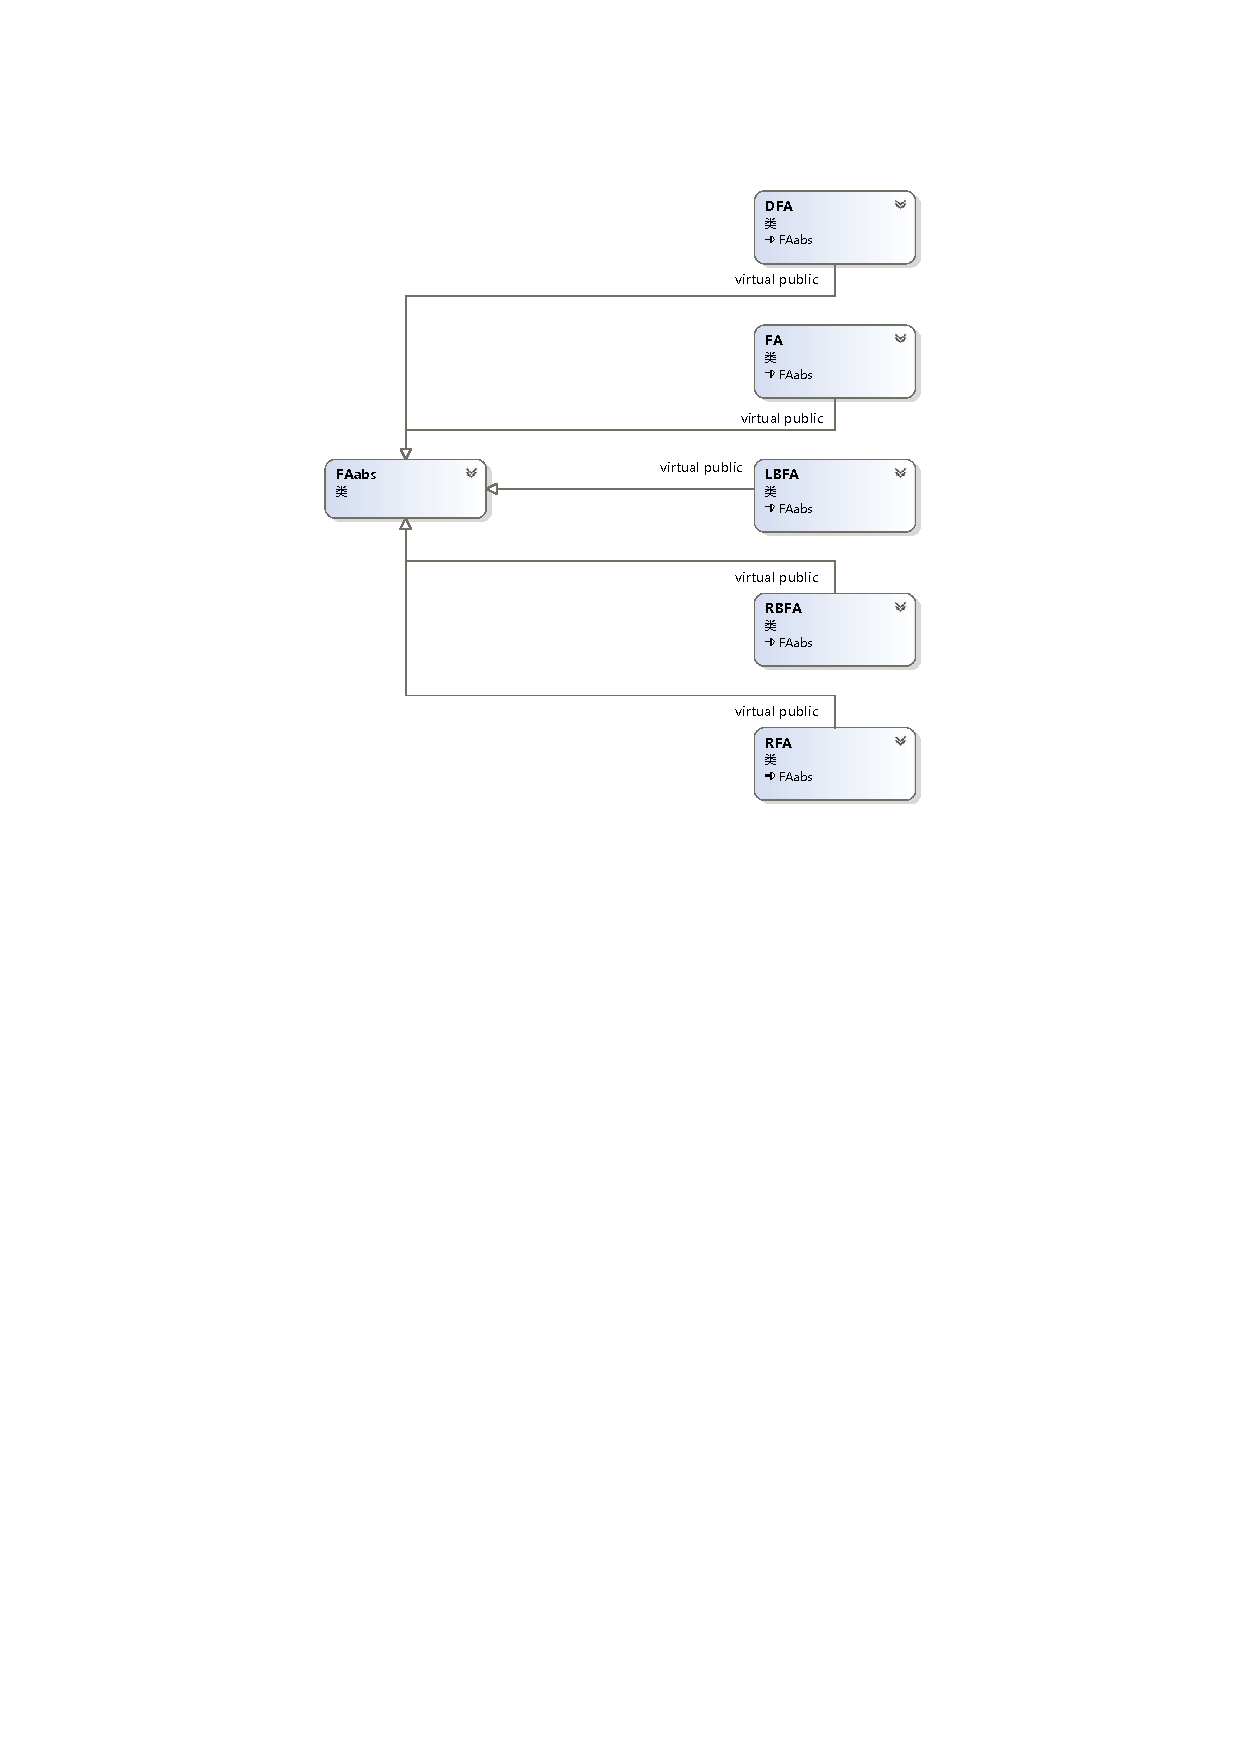
\includegraphics[width=0.7\textwidth]{FAabsRel}
    \caption{类FAabs及其派生类}
    \label{fig:FAabsRel}
\end{figure}

\section{DFA类}
在本文中,我们仅仅对 DFA 应用最小化算法,FIRE engine 提供了多种方式构造一个 DFA,要得到一个类 DFA 的对象,在已经实例化类 FA 、类 RFA 、类 RBFA 或类 LBFA 的情况下, 可以通过执行他们的成员成员函数 “determinism()” 得到一个类 DFA 对象。


类 DFA 的部分实现如表 \ref{tab:Class-DFA} 

\begin{table}[!htbp]
    \caption{类 DFA}
    \label{tab:Class-DFA}
    \centering
    \small% fontsize
    \setlength{\tabcolsep}{4pt}% column separation
    \renewcommand{\arraystretch}{1.2}%row space 
    %\begin{tabular}{lcrr} 
        \begin{tabular}{llll} %l p{4em}<{\centering} p{3em}<{\centering} p{3em}<{\centering}
        \toprule 
         \multicolumn{4}{c}{Class DFA} \\
        \midrule
        名称& 类型 & 属性  &\mbox{说明} \\
        \midrule
        Q & StatePool & protected &          \\
        S & StateSet  & protected &  $S\subseteq Q$ \\
        F & StateSet  & protected &  $F\subseteq Q$\\
        T & DTransRel & protected &  转移关系\\
        \midrule 
        DFA(const DFA\_components\& r);& & public &构造函数 \\
        reconstruct(const DFA\_components\& r); & DFA\& & public & \\
        determinism() const; & DFA & public & \\
        reverse(); & DFA\& & public & 反转 DFA \\
        min\_Brzozowski(); & DFA\& & public & 最小化算法 \\
        min\_HopcroftUllman(); & DFA\& & public & 最小化算法 \\
        min\_dragon(); & DFA\& & public & 最小化算法 \\
        min\_Hopcroft(); & DFA\& & public & 最小化算法 \\
        min\_Watson(); & DFA\& & public & 最小化算法 \\
        usefulf(); & DFA\& & public &  \\
        split(State,State,CharRange,StateEqRel\&); & State & public & 分割等价类 \\
        \bottomrule 
    \end{tabular}
\end{table}


由表 \ref{tab:Class-DFA} 可知,类$DFA$默认情况下,提供一个用“DFA\_components”变量的引用来实例化DFA对象的方法。






%\newpage
\section{DFA\_components 结构体}\label{sc:dfa_com}% ~\label{sc:dfa_com}

从“DFA\_components”构造一个$DFA$对象是最简单直接的方法,观察“DFA\_components”的实现,如表\ref{tab:DFA-components}所示
\begin{table}[!htbp]
    \caption{结构体 DFA\_components}
    \label{tab:DFA-components}
    \centering
    \small% fontsize
    \setlength{\tabcolsep}{4pt}% column separation
    \renewcommand{\arraystretch}{1.2}%row space 
    %\begin{tabular}{lcrr} 
        \begin{tabular}{p{3em}<{\centering} p{5em}<{\raggedright} p{5em}<{\raggedright}} %l p{4em}<{\centering} p{3em}<{\centering} p{3em}<{\centering}
        \toprule 
         \multicolumn{3}{c}{struct DFA\_components} \\
        \midrule
        名称& 类型 & \mbox{说明} \\
        \midrule
        Q & StatePool &           \\
        S & StateSet  &  $S\subseteq Q$ \\
        F & StateSet  &  $F\subseteq Q$ \\
        T & DTransRel &  转移关系  \\
        \bottomrule
    \end{tabular}
\end{table}

由表\ref{tab:DFA-components}可知,结构体 DFA\_components 内包含 StatePool 变量$Q$, StateSet 变量$S$, DTransRel 变量$T$, StateSet 变量$F$。若需要声明一个 DFA\_components 变量,则需要分别实例化 StatePool 、StateSet、DTransRel对象。这几个类还分别继承自其他的类,如图 \ref{fig:DFARel} 所示。

\begin{figure}[!htbp]
    \centering
    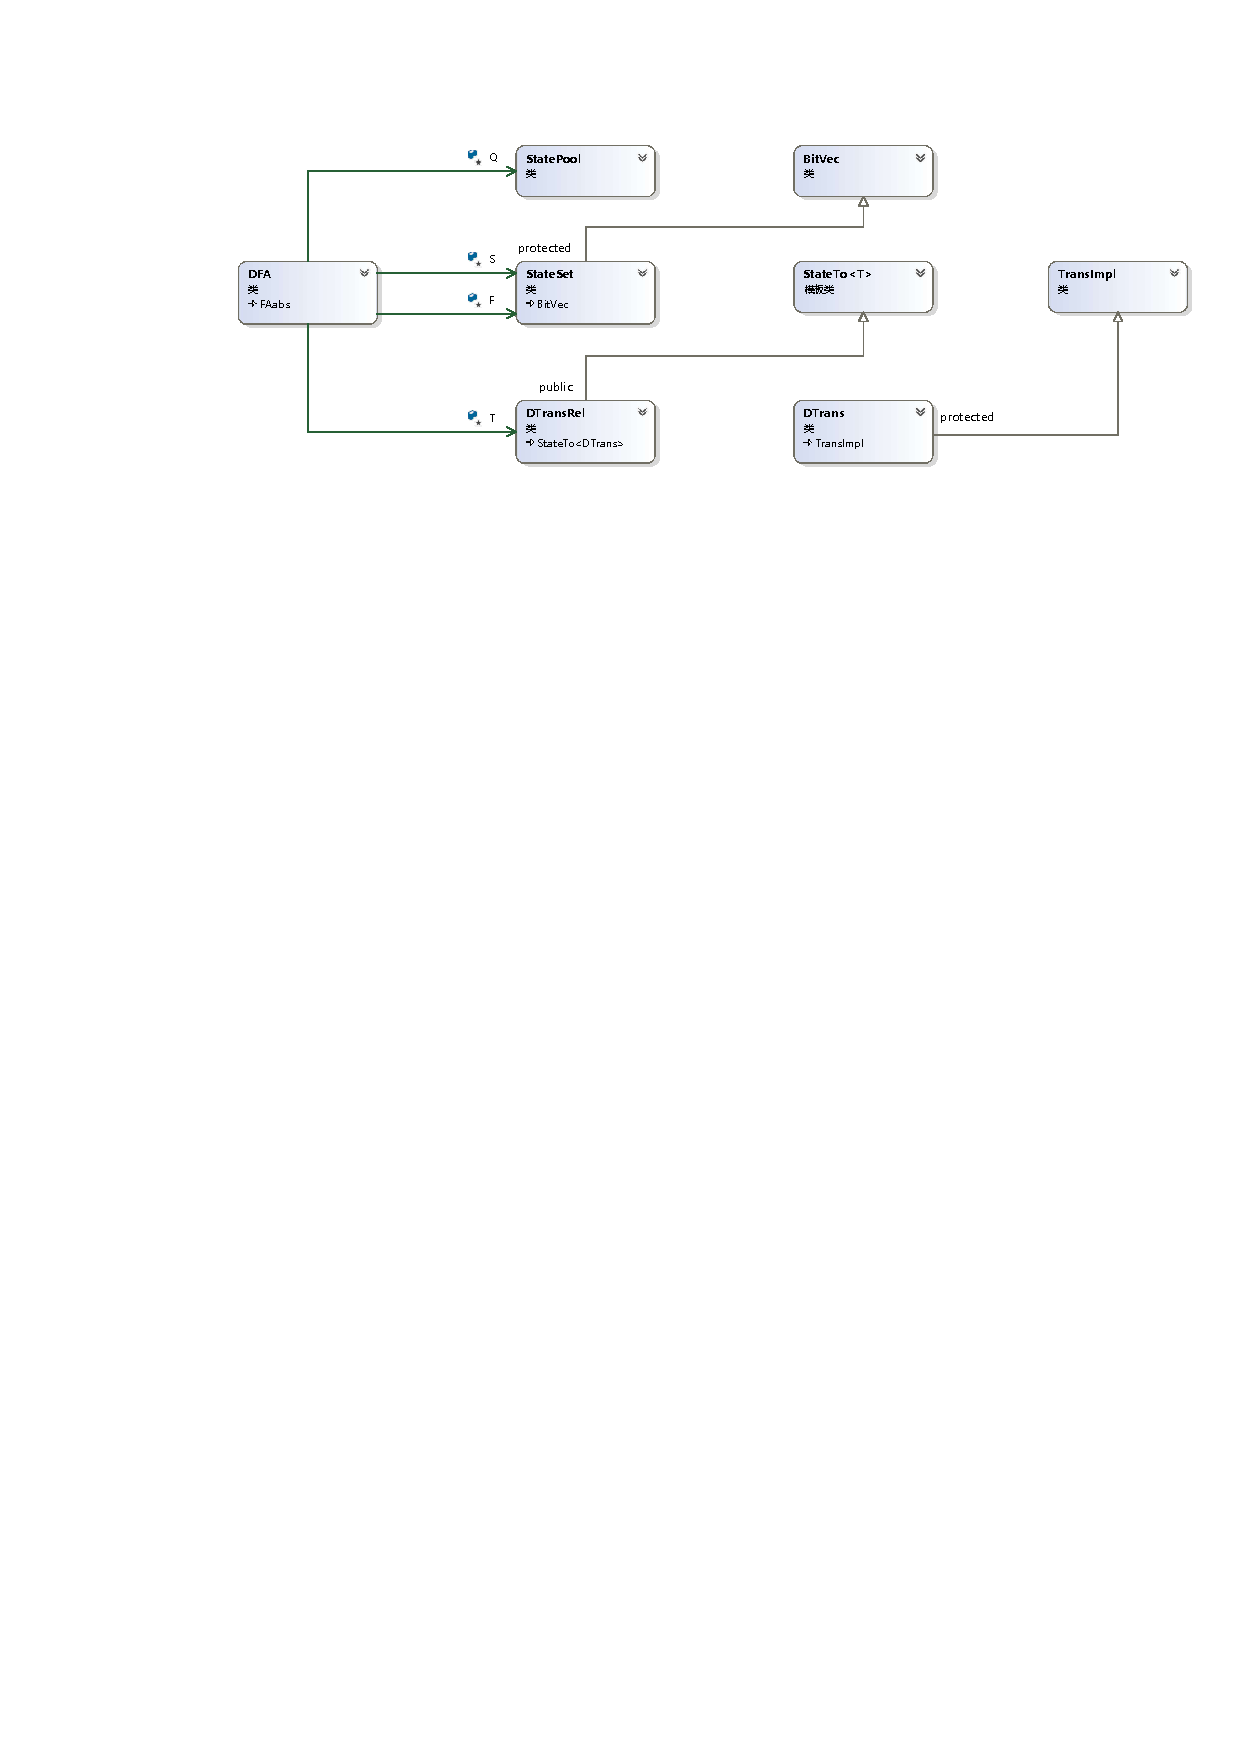
\includegraphics[width=\textwidth]{DFARel}
    \caption{DFA与其成员类及成员类的基类}
    \label{fig:DFARel}
\end{figure}

类 DFA 的成员变量 “T” 为一个 DTransRel 对象,公有继承自模板类 StateTo<T>,模板参数 “T” 为保护继承自类 TransImpl 的类 DTrans 。

\subsection{StatePool 类}
StatePool类的部分实现如表 \ref{tab:Class-StatePool} (文件$StatePool.h$):
% \lstset{style=mystyle}
% \begin{lstlisting}[language=C++,label={lst:StatePool},caption={StatePool}]
% class StatePool
% {
% public:
%     // How many states are already allocated(one more than that last allocated one,
%     // since it begins at 0).
%     inline int size() const;
%     ……
%     // Allocate a new state.
%     inline State allocate();
%     ……
% private:
%     // The next one to be allocated.
%     int next;
% };
% ……
% inline int StatePool::size() const
% {
%     return(next);
% }
% ……
% inline State StatePool::allocate()
% {
%     return(next++);
% }
% \end{lstlisting}

\begin{table}[!htbp]
    \caption{类 StatePool}
    \label{tab:Class-StatePool}
    \centering
    \small% fontsize
    \setlength{\tabcolsep}{4pt}% column separation
    \renewcommand{\arraystretch}{1.2}%row space 
    %\begin{tabular}{lcrr} 
        \begin{tabular}{llll} %l p{4em}<{\centering} p{3em}<{\centering} p{3em}<{\centering}
        \toprule 
         \multicolumn{4}{c}{Class StatePool} \\
        \midrule
        名称& 类型 & 属性  &\mbox{说明} \\
        \midrule
        next & int & private &          \\
        \midrule 
        StatePool(const StatePool\& r);& & public &构造函数 \\
        size() const; & int & public & \\
        allocate();  &   State &  public & \\
        set\_domain(const\ int r); & int & public & \\
        contains(const State r) const; & int & public & \\
        \bottomrule 
    \end{tabular}
\end{table}
如表 \ref{tab:Class-StatePool} 所示,其中 StatePool::size() 和 StatePool::allocate() 为类 StatePool 两个比较重要的函数,前者为自动机 $M$ 的大小,也即 $|M|=|Q|$。 StatePool::allocate() 用来向 StatePool 增加新的状态。
\subsection{StateSet 类}
类$StateSet$的部分声明如表 \ref{tab:Class-StateSet}(文件$StateSet.h$):
% \lstset{style=mystyle}
% \begin{lstlisting}[language=C++,label={lst:StateSet},caption={StateSet}]
% class StateSet :protected BitVec
% {
% public:
% ……
%     // inserts a State. r = [0,domain())
%     inline StateSet& add(const State r);
    
%     // set How many States can this set contain.
%     // [O, r) can be contained in *this.
%     inline void set_domain(const int r);
% ……
% }
% \end{lstlisting}

\begin{table}[!htbp]
    \caption{类 StateSet}
    \label{tab:Class-StateSet}
    \centering
    \small% fontsize
    \setlength{\tabcolsep}{4pt}% column separation
    \renewcommand{\arraystretch}{1.2}%row space 
    %\begin{tabular}{lcrr} 
        \begin{tabular}{llll} %l p{4em}<{\centering} p{3em}<{\centering} p{3em}<{\centering}
        \toprule 
         \multicolumn{4}{c}{Class StateSet : protected BitVec} \\
        \midrule
        名称& 类型 & 属性  &\mbox{说明} \\
        \midrule 
        StateSet(); &  &  public & 构造函数 \\
        empty() const; & int & public & \\
        size() const;  & int & public & \\
        complement();  & StateSet\& & public & 求补集 \\
        add(const State r);  & StateSet\& & public &  \\
        remove(const State r);  & StateSet\& & public &  \\
        set\_union(const StateSet\& r);  & StateSet\& & public & 求并集 \\
        intersection(const StateSet\& r);  & StateSet\& & public & 求交集 \\
        remove(const StateSet\& r);  & StateSet\& & public &  \\
        smallest() const; & State & public & \\
        set\_domain(const int r); & void & public & \\
        \bottomrule 
    \end{tabular}
\end{table}

由于在实例化过程$DFA$对象的过程中,只需要用到类 StateSet 的成员函数 StateSet::set\_domain() 和 StateSet::add() 。类 StateSet 中有集合的交、并、差、补、判断是否为空集等功能,这些功能实际上由类 State 的父类 BitVec 提供,这里不再赘述类 BitVec 的内容。


\subsection{DTransRel 类}

类$DTransRel$是$DFA$的一个重要成员,它存储了$DFA$的状态转移关系,最小化算法中用到的等价类分割、等价状态合并等功能都与这个类息息相关。类 DTransRel 的部分实现如表 \ref{tab:Class-DTransRel} 所示(文件$DTransRel.h$):
% \lstset{style=mystyle}
% \begin{lstlisting}[language=C++,label={lst:DTransRel},caption={DTransRel}]
% // Implement a deterministic transition relation, as a function from States time
% // char to State.This is used for transition relations in DFA's.
% class DTransRel :public StateTo<DTrans>
% {
% public:
% ……
%     // Some functions updating *this:
%     inline DTransRel& add_transition(const State p, const CharRange a, const State q);
% ……
%     // Change the domain of this relation.
%     inline void set_domain(const int r);
% ……
% }
% \end{lstlisting}

\begin{table}[!htbp]
    \caption{类 DTransRel}
    \label{tab:Class-DTransRel}
    \centering
    \small% fontsize
    \setlength{\tabcolsep}{4pt}% column separation
    \renewcommand{\arraystretch}{1.2}%row space 
    %\begin{tabular}{lcrr} 
        \begin{tabular}{llll} %l p{4em}<{\centering} p{3em}<{\centering} p{3em}<{\centering}
        \toprule 
         \multicolumn{4}{c}{class DTransRel :public StateTo<DTrans>} \\
        \midrule
        名称& 类型 & 属性  &\mbox{说明} \\
        \midrule 
        DTransRel(); &  &  public & 构造函数 \\
        image(const State r, const char a) const; & State & public & \\
        transition\_on\_range(State r, CharRange a) const; & State & public & \\
        reverse\_transition(const State r, const CharRange a) const; & StateSet & public & \\
        labels\_between(const State r, const StateSet\& s) const; & CRSet & public & \\
        out\_labels(const State r) const; & CRSet & public & \\
        reverse\_closure(const StateSet\& r) const; & StateSet & public & \\
        add\_transition(State p, CharRange a, State q); & DTransRel\& & public & \\
        set\_domain(const int r); & void & public & \\
        \bottomrule 
    \end{tabular}
\end{table}

在实例化类 DFA 的过程中,类 DTransRel 需要用到的成员函数只有 DTransRel::set\_domain() 和 DTransRel::add\_transition() 。







%%%%%%%%%%%%%%%%%%%%%%%%%%%%%%%%%%%%%%%%%%%%%%%%%%%%%%%%%%%%%%%%%%%%%%%%%%%%%%%%%%%%%%%%%%%%%%%%%%%%%%%%%%%%%%%%%%%%%%
\section{实例化类DFA对象}\label{sec:get_a_dfa}

在文件$DFA.cpp$中有如下实现:

\begin{lstlisting}[language=C++,label={lst:DFACpp},caption={DFA.cpp}]
inline int DFA::class_invariant() const
{
	return(Q.size() == S.domain()
		&& Q.size() == F.domain()
		&& Q.size() == T.domain()
		&& current < Q.size()
		&& S.size() <= 1);
}
\end{lstlisting}
而文件$DFA.h$中的构造函数如下:

\begin{lstlisting}[language=C++,label={lst:DFA_H},caption={DFA.h}]
inline DFA::DFA(const DFA_components& r) :Q(r.Q), S(r.S), F(r.F), T(r.T)
{
	current = Invalid;
	assert(class_invariant());
}
\end{lstlisting}
由代码 \ref{lst:DFACpp} 和代码 \ref{lst:DFA_H} 可知,在语句 “assert(class\_invariant());” 处,若函数 “class\_invariant()” 返回值为 “false”,那么程序将在此处中止\cite{assert_abort}(下称 assert 中止)。由此可以知道,类$DFA$要求其成员变量满足
\begin{equation}\label{eq:DFA_class_invariant}
    (Q.size() \equiv S.domain() \equiv T.domain ) \land (S.size() \leq 1)
\end{equation}
对于$current \le Q.size() $,“current”变量的值被初始化为“Invalid”,并且之后没有对其进行更改,所以不列入式\ref{eq:DFA_class_invariant}中。

在文件$State.h$中有如下定义

\begin{lstlisting}[language=C++,label={lst:State_H},caption={State.h}]
// Encode automata states as integers.
typedef signed int State;

// Invalid states mean something bad is about to happen.
const State Invalid = -1;
\end{lstlisting}
由代码\ref{lst:State_H}可知,$State$类型实际上是整型,而“Invalid”为“-1”。

%\clearpage
根据本节以上内容以及\ref{sc:dfa_com}节内容所说,可以实例化如图\ref{fig:DFA1}的自动机。

\begin{figure}[!htbp]
    \centering
    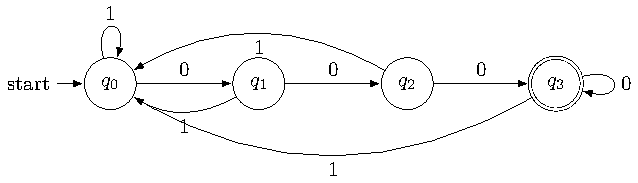
\includegraphics[width=0.7\textwidth]{automaton_1}
    \caption{DFA示例}
    \label{fig:DFA1}
\end{figure}

\newpage
图\ref{fig:DFA1}中的自动机的转移函数如表\ref{tab:DFA1}

\begin{table}[!htbp]
    \caption{图{\ref{fig:DFA1}}状态转移函数}
    \label{tab:DFA1}
    \centering
    \small% fontsize
    \setlength{\tabcolsep}{4pt}% column separation
    \renewcommand{\arraystretch}{1.2}%row space 
    \begin{tabular}{l p{3em}<{\centering} p{3em}<{\centering} p{3em}<{\centering}}
        \toprule %\hline 
        \multirow{2}{*}{状态说明} & \multirow{2}{*}{状态} & \multicolumn{2}{c}{输入字符} \\
		\cline{3-4}      &    &$0$ & $1$  \\
        \midrule%\hline
        开始状态(start)          & $q_0$ & $q_1$  & $q_0$    \\
                                & $q_1$ & $q_2$  & $q_0$    \\
                                & $q_2$ & $q_3$  & $q_0$    \\
        结束状态(final)         & $q_3$ & $q_3$  & $q_0$    \\
        \bottomrule%\hline  
    \end{tabular}
\end{table}

实例化$DFA$类如代码\ref{lst:DFASample}:

% \lstset{style=mystyle}
% \begin{lstlisting}[language=C++,label={lst:DFASample},caption={实例化DFA示例}]
% #include"DFA.h"
% #include<iostream>
% int main()
% {
%     DFA_components dfa_com1;

%     // StateSet S  开始状态集
%     dfa_com1.S.set_domain(10);
%     dfa_com1.S.add(0);

%     // StateSet F  结束状态集
%     dfa_com1.F.set_domain(10);
%     dfa_com1.F.add(3);

%     // StatePool Q 
%     int i = 10;
%     while (i--)
%     {
%         dfa_com1.Q.allocate();
%     }

%     // DTransRel T transition             
%     dfa_com1.T.set_domain(10);
%     dfa_com1.T.add_transition(0, '0', 1);
%     dfa_com1.T.add_transition(1, '0', 2);
%     dfa_com1.T.add_transition(2, '0', 3);
%     dfa_com1.T.add_transition(3, '0', 3);
%     dfa_com1.T.add_transition(0, '1', 0);
%     dfa_com1.T.add_transition(1, '1', 0);
%     dfa_com1.T.add_transition(2, '1', 0);
%     dfa_com1.T.add_transition(3, '1', 0);

%     DFA dfa1(dfa_com1);
%     dfa1.usefulf();

%     std::cout<<dfa1<<std::endl;
	
%     return 0;
% }
% \end{lstlisting}

代码 \ref{lst:DFASample} 将在控制台输出如下信息:

\begin{lstlisting}[language=C++,label={lst:DFASampleLog},caption={图\ref{fig:DFA1}中自动机在 FIRE engine 中的表现形式}]
DFA
Q = [0,4)
S = { 0 }
F = { 3 }
Transitions =
0->{ '0'->1  '1'->0 }
1->{ '0'->2  '1'->0 }
2->{ '0'->3  '1'->0 }
3->{ '0'->3  '1'->0 }

current = -1
\end{lstlisting}

下文中将以表 \ref{tab:DFA1} 的形式来描述一个自动机,以代码 \ref{lst:DFASampleLog} 的形式来表示自动机在 FIRE engine 中的展现形式。实例化一个 DFA 时以 “实例化 DFA” 代指,不用代码表示。 